%#!uplatex

\documentclass[a4paper,dvipdfmx,openany,uplatex,report]{jsbook} % 卒論用クラス

\usepackage{style/thesis} % 卒論用スタイル

% ----------
% 基本情報
% ----------
\thesistype{卒業論文}                              % 論文種別
\title{卒業論文のテンプレートと書き方ガイド}          % タイトル
\subtitle{}                                       % サブタイトル（不要なら空のまま）
\author{X12345\quad 愛工太郎}                       % 著者（学籍番号 氏名）
\supervisor{小栗真弥}                               % 指導教員
\affiliation{愛知工業大学\quad 情報科学部\quad 情報科学科} % 所属
\date{2026年3月}                                   % 提出年月

% ----------

\begin{document}
    \ThisIsDraft % 下書きの時はこれをつけるとバージョン管理ができます

    % ===== 前付け（表紙・目次） =====
    \frontmatter
    \maketitle
    \tableofcontents
    \listoffigures
    % \listoftables
    % \listoftodos

    % ===== 本文 =====
    \mainmatter
    \chapter{序論}
\label{chap:intro}

本章は，卒業論文・修士論文における「序論（はじめに）」の書き方を実例として示すものである．
序論は読者が最初に目にする章であり，論文全体の印象を大きく左右する．
一般に，\textbf{研究背景}・\textbf{問題提起}・\textbf{研究目的}・\textbf{論文の構成}の順に記述するとよい\cite{kisaragi}．
本章自体がその構成例になっている．

%% ===========================================================
\section{研究の背景}
\label{sec:background}
まず，研究対象とする分野の現状や社会的な背景を述べ，読者を研究テーマへ導く．
本テンプレートは，\upLaTeX\footnote{\LaTeX を日本語（特に縦書きや多書体）に対応させた処理系である．}
を用いて論文を執筆するための環境を提供する．
組版システムとしての\TeX は文献\cite{lamport}や文献\cite{tex}をはじめ多くの文献で解説されており，
学術論文の作成において広く利用されている．

背景の記述では，専門外の読者にも伝わるように，一般的な事柄から具体的な対象へと
順に話を進めることが望ましい．略語を用いる場合は初出時に正式名称を併記する
（例：自然言語処理 (Natural Language Processing; NLP)）．

%% ===========================================================
\section{既存研究の課題}
\label{sec:problem}
次に，既存の手法や状況にどのような課題があるのかを示す．
ここでの問題提起が，後の研究目的と対応している必要がある．
課題を述べる際は，単なる感想ではなく，先行研究の引用\cite{tex,kisaragi}に基づいて
客観的に論じることが重要である．

%% ===========================================================
\section{本研究の目的}
\label{sec:purpose}
問題提起を受けて，本研究が何を目指すのかを明確に述べる．
目的が曖昧であったり，問題提起と対応していなかったりする論文は再考を要する．
本テンプレートの目的は，論文の体裁を整える手間を最小化し，
執筆者が内容の検討に集中できる環境を提供することである．

%% ===========================================================
\section{本論文の構成}
\label{sec:structure}
最後に，以降の章で何を述べるのかを示す．
読者はこの記述を地図として論文を読み進める．

\begin{description}
    \item[第\ref{chap:intro}章\ 序論] 研究の背景・課題・目的と，本論文の構成を述べる（本章）．
    \item[第\ref{chap:writing}章\ 論文執筆の作法] 論文全体の構成や，わかりやすい文章を書くための作法をまとめる．
    \item[第\ref{chap:latex}章\ 文章作成のための\LaTeX 記法] 見出し・参照・箇条書き・引用など，文章を組み立てる基本的な記法を示す．
    \item[第\ref{chap:float}章\ 図・表・数式・コードの記法] 図の載せ方や表・数式・ソースコードなど，論文で多用する記法をパターン豊富に示す．
    \item[第\ref{chap:conclusion}章\ 結論] 本論文のまとめと今後の課題を述べる．
\end{description}

\begin{itembox}[l]{序論に含めるべき要素}
    \begin{enumerate}
        \item 研究背景：分野の現状や社会的背景
        \item 問題提起：既存手法・状況の課題
        \item 研究目的：課題に対して本研究が目指すこと
        \item 論文の構成：以降の章の概要
    \end{enumerate}
\end{itembox}

    \chapter{論文執筆の作法}
\label{chap:writing}

本章では，論文を執筆する上での作法をまとめる．
内容・体裁ともにしっかりした論文を書くために，全体の構成から文章表現の細部までを順に説明する．

%% ===========================================================
\section{論文全体の構成}
\label{sec:overall-structure}
論文は，読者が研究の流れを追えるように章を構成する．
実験を伴う研究では，いわゆる IMRAD（Introduction, Methods, Results, and Discussion）型の構成が
よく用いられる．一般的な章構成の例を以下に示す．

\begin{enumerate}
    \item 序論（研究背景・問題提起・目的・論文の構成）
    \item 関連研究（先行研究の整理と本研究の位置づけ）
    \item 提案手法（本研究で提案する手法やシステムの説明）
    \item 評価・実験（実験条件・結果・考察）
    \item 結論（成果のまとめと今後の課題）
\end{enumerate}

上記はあくまで一例であり，研究内容に応じて適切な構成を考えること．
章・節の構成が不適切な論文は，読者にとって大きな負担となる\cite{kisaragi}．

%% ===========================================================
\section{各章の役割と書き方}
\label{sec:each-chapter}

\subsection{序論}
研究の背景と課題を示し，本研究の目的を明確にする．
第\ref{chap:intro}章がその記述例である．

\subsection{関連研究}
本研究に関連する先行研究を整理し，それらとの違いや本研究の新規性を述べる．
既知の技術が何であり，何を新しいアイデアとして提案しているのかを明確にする必要がある．
十分な文献調査と引用は，新規性の主張に欠かせない．

\subsection{提案手法}
提案する手法やシステムを，読者が再現できる程度に具体的に説明する．
概念的・抽象的な説明に終始し，読者が具体的な内容を理解できないものは再考を要する．
図や数式，アルゴリズムを適切に用いて説明するとよい（第\ref{chap:latex}章参照）．

\subsection{評価・実験}
提案手法の有効性を，実験や評価によって客観的に示す．
実験条件を明記し，結果を表やグラフで提示したうえで，その結果が何を意味するのかを考察する．
有効性の主張がない，または極めて貧弱なものは再考を要する．

\subsection{結論}
本研究で行ったことと得られた成果を簡潔にまとめる．
序論で述べた目的に対してどの程度達成できたかを振り返り，今後の課題や展望を述べる．

%% ===========================================================
\section{わかりやすい文章の作法}
\label{sec:writing-style}
研究の新規性・有用性・信頼性が読者に伝わるように記述する\cite{kisaragi}．
読み手にとって読みやすい文章を心がけ，以下の点に注意する．

\begin{itemize}
    \item 「だ・である」調（常体）で統一する．「です・ます」調と混在させない
    \item 一文は短く簡潔にする．極端な口語体や長文の連続は避ける
    \item 主語と述語の対応を明確にする．長い文は主述がねじれやすい
    \item 曖昧な表現（「〜と思われる」「〜的な」）を避け，根拠に基づいて記述する
    \item 指示語（「これ」「それ」）の指す内容が一意に定まるようにする
    \item 説明に飛躍がないか，逆に冗長すぎる部分がないかを確認する
    \item 未定義の用語を減らし，専門用語には適切な説明を付ける
\end{itemize}

%% ===========================================================
\section{句読点と文字の使い分け}
\label{sec:punctuation}
句点には全角の「．」，読点には全角の「，」を用いる（本テンプレートの慣例）．
ただし英文中や数式中では半角の「.」「,」を用いる．「。」「、」は使用しない．

全角文字と半角文字の使い分けは以下の通りである．
\begin{itemize}
    \item 英数字・空白・記号類は半角文字を用いる
    \item カタカナは全角文字を用いる
    \item 括弧は全角の「（）」を基本とし，英文中では半角の「()」を用いる
    \item 引用符は開きと閉じを区別する．開きには\,``\,を，閉じには\,''\,を用いる
\end{itemize}

%% ===========================================================
\section{引用のマナー}
\label{sec:citation-manner}
他者の研究成果や主張を利用する際は，必ず出典を明記する．
出典を示さずに引用することは剽窃であり，固く禁じられている．
本文中での引用には\verb|\cite{}|を用い，引用した文献のみを参考文献リストに列挙する
（記法の詳細は第\ref{sec:reference}節を参照）．

%% ===========================================================
\section{図表の扱い方}
\label{sec:figure-manner}
図表には必ずキャプションを付け，本文中で参照すること．
使用していない図表を掲載してはならない．また，図は原則として自分で作成したものを用いる．
標準テストイメージ等を除き，他者が作成した図表を引用の明示なく用いることは禁止である．
具体的な作成方法は第\ref{sec:figure}節および第\ref{sec:table}節で述べる．

%% ===========================================================
\section{生成AIの利用について}
\label{sec:ai}
ChatGPTやGemini，Claude等の生成AIは，文章の推敲やアイデアの整理など，
執筆を補助するツールとして活用できる．ただし，以下の点に十分注意すること．

\begin{itemize}
    \item 生成AIの出力をそのまま貼り付けてはならない．内容を吟味し，自らの文章として記述する
    \item 生成AIは事実と異なる内容（ハルシネーション）を生成することがある．出力内容は必ず裏付けを取ること
    \item 存在しない参考文献を生成することがあるため，引用情報は必ず原典にあたって確認する
    \item 生成AIの利用方針は指導教員や学科の指示に従うこと
\end{itemize}
内容の責任は著者自身が負うことを忘れてはならない．

%% ===========================================================
\section{推敲と提出前チェック}
\label{sec:proofreading}
論文は必ず提出前に指導教員の確認を受けること．
締切直前にいきなり見せるのではなく，早い段階から計画的に執筆を進め，
フィードバックを受けて改良を重ねる．同級生や先輩に読んでもらうことも有効である．

提出前には以下の点を最終確認する\cite{ipsj-sample}．
\begin{itemize}
    \item \verb|\ThisIsDraft|が削除またはコメントアウトされているか
    \item タイトル・氏名・指導教員名に誤りがないか
    \item 図表番号・参考文献番号が正しく参照されているか（未参照・未定義がないか）
    \item フォントが埋め込まれているか（印刷時の文字化けを防ぐ）
    \item overfull が発生していないか（第\ref{sec:overfull}節参照）
\end{itemize}

    \chapter{文章作成のための\LaTeX 記法}
\label{chap:latex}

本章と次章では，論文の執筆に必要な\LaTeX の記法を，さまざまなパターンとともに丁寧に示す．
各項目では，可能な限り実際の出力と対応するソースコードを併記する．
本章では文章を組み立てるための基本的な記法を，
第\ref{chap:float}章では図・表・数式・ソースコードの記法を扱う．

%% ===========================================================
\section{文書の構造と見出し}
\label{sec:sectioning}
論文の見出しは，以下の階層で構成する．数字が小さいほど上位の見出しである．

\begin{enumerate}[label=\arabic*., leftmargin=*]
    \item \verb|\chapter{...}|：章（本テンプレートの最上位）
    \item \verb|\section{...}|：節
    \item \verb|\subsection{...}|：小節
    \item \verb|\subsubsection{...}|：小々節
    \item \verb|\paragraph{...}|：段落見出し（番号なし・行内）
\end{enumerate}

見出しに\verb|*|を付けると番号が振られず，目次にも載らない（例：\verb|\section*{...}|）．
「はじめに」や「謝辞」など，番号を付けたくない見出しに用いる．
番号を付ける深さは\verb|secnumdepth|，目次に載せる深さは\verb|tocdepth|カウンタで調整できる．

\begin{lstlisting}[language={[LaTeX]TeX}, numbers=none, frame=single]
\setcounter{secnumdepth}{2} % subsection まで番号を振る
\setcounter{tocdepth}{2}    % subsection まで目次に載せる
\end{lstlisting}

%% ===========================================================
\section{相互参照}
\label{sec:crossref}
見出し・図・表・式などに\verb|\label{key}|を付けておくと，
\verb|\ref{key}|で番号を，\verb|\pageref{key}|でページ番号を参照できる．
番号を手書きする必要がなくなり，順序が変わっても自動で更新される．

\begin{table}[htbp]
    \centering
    \caption{主な参照コマンド}
    \label{tab:refcmd}
    \begin{tabular}{ll}\toprule
        コマンド & 用途 \\ \midrule
        \verb|\ref{key}|     & 章・節・図・表・式などの番号 \\
        \verb|\pageref{key}| & 対象があるページ番号 \\
        \verb|\eqref{key}|   & 式番号（括弧付き，例：(\ref{eq:dummy})） \\
        \verb|\autoref{key}| & 種別付きの参照（hyperref，例：「図1」） \\
        \verb|\label{key}|   & 参照先に目印を付ける \\ \bottomrule
    \end{tabular}
\end{table}

\begin{equation}\label{eq:dummy} E = mc^2 \end{equation}

ラベルのキーには，種別を表す接頭辞を付けると管理しやすい
（章：\verb|chap:|，節：\verb|sec:|，図：\verb|fig:|，表：\verb|tab:|，式：\verb|eq:|，コード：\verb|lst:|）．
たとえば本節（第\ref{sec:crossref}節）は\pageref{sec:crossref}ページにあり，式は\eqref{eq:dummy}である．

%% ===========================================================
\section{文字の書体と装飾}
\label{sec:fontstyle}
文字の見た目は表\ref{tab:fontstyle}のコマンドで変更できる．
論文では装飾を多用せず，強調は\verb|\textbf{}|か\verb|\emph{}|に絞るのがよい．

\begin{table}[htbp]
    \centering
    \caption{書体・装飾のコマンド}
    \label{tab:fontstyle}
    \begin{tabular}{lll}\toprule
        コマンド & 出力 & 用途 \\ \midrule
        \verb|\textbf{...}|  & \textbf{太字}            & 強調 \\
        \verb|\textit{...}|  & \textit{italic}          & 欧文の斜体 \\
        \verb|\emph{...}|    & \emph{強調}              & 文脈に応じた強調 \\
        \verb|\texttt{...}|  & \texttt{typewriter}      & 等幅（コード等） \\
        \verb|\textsf{...}|  & \textsf{sans serif}      & サンセリフ \\
        \verb|\underline{}|  & \underline{下線}         & 下線 \\
        \verb|{\gtfamily }|  & {\gtfamily ゴシック体}   & 和文ゴシック \\
        \verb|{\mcfamily }|  & {\mcfamily 明朝体}       & 和文明朝 \\ \bottomrule
    \end{tabular}
\end{table}

文字サイズは\verb|\tiny|，\verb|\small|，\verb|\normalsize|，\verb|\large|，
\verb|\Large|，\verb|\huge|の順に大きくなる（例：{\large 大きめ}，{\small 小さめ}）．
これらは宣言型なので，\verb|{\large ... }|のように波括弧で範囲を限定する．

%% ===========================================================
\section{空白・改行・改ページ}
\label{sec:spacing}
\LaTeX では，ソース中の単語間の複数の空白や単独の改行は，1つの空白として扱われる．
空行を入れると段落の区切り（改段落）になる．主な制御コマンドを以下に示す．

\begin{description}[leftmargin=*, style=nextline]
    \item[\texttt{\textbackslash\textbackslash}\ または\ \texttt{\textbackslash newline}] 段落内で強制改行する（多用は避ける）．
    \item[\texttt{\textbackslash par}\ または空行] 段落を改める．
    \item[\texttt{\textbackslash noindent}] 段落先頭の字下げを無くす．
    \item[\texttt{\textbackslash newpage},\ \texttt{\textbackslash clearpage}] 改ページする（\verb|\clearpage|は未処理の図表も出力する）．
    \item[\texttt{\textbackslash quad},\ \texttt{\textbackslash qquad}] 全角1文字・2文字分の水平空白を入れる．
    \item[\texttt{\textbackslash hspace\{1cm\}},\ \texttt{\textbackslash vspace\{1cm\}}] 任意の幅・高さの空白を入れる．
\end{description}

文字間に\verb|~|を書くと改行されない空白（ノーブレークスペース）になり，
「図~1」のように番号と語句が行末で泣き別れになるのを防げる．

%% ===========================================================
\section{特殊文字と記号}
\label{sec:special}
\LaTeX で特別な意味を持つ文字は，そのまま書くとエラーになるためエスケープが必要である（表\ref{tab:special}）．

\begin{table}[htbp]
    \centering
    \caption{特殊文字の入力方法}
    \label{tab:special}
    \begin{tabular}{cl@{\qquad}cl}\toprule
        出力 & 入力 & 出力 & 入力 \\ \midrule
        \% & \verb|\%|  & \&         & \verb|\&| \\
        \$ & \verb|\$|  & \#         & \verb|\#| \\
        \_ & \verb|\_|  & \{\ \}     & \verb|\{ \}| \\
        \textasciitilde & \verb|\textasciitilde| & \textasciicircum & \verb|\textasciicircum| \\
        \textbackslash  & \verb|\textbackslash|  & \ldots           & \verb|\ldots| \\ \bottomrule
    \end{tabular}
\end{table}

ハイフンには3種類ある：ハイフン（-，\verb|-|），
半角ダッシュ（--，\verb|--|，範囲を表す），全角ダッシュ（---，\verb|---|，欧文の挿入句）．
欧文の引用符は，開きに\verb|``|，閉じに\verb|''|を用いる（``例''）．

%% ===========================================================
\section{箇条書き}
\label{sec:lists}
箇条書きには\texttt{itemize}（記号），\texttt{enumerate}（番号），
\texttt{description}（見出し付き）の3種類がある．これらは入れ子にできる．

\begin{itemize}
    \item itemize は記号付き
    \begin{itemize}
        \item 入れ子にすると記号が変わる
        \begin{itemize}
            \item さらに入れ子にもできる
        \end{itemize}
    \end{itemize}
    \item enumerate は番号付き
\end{itemize}

\texttt{enumitem}パッケージを使うと，番号やラベルの書式・余白を細かく変更できる．

\begin{enumerate}[label=(\arabic*), leftmargin=*]
    \item \verb|label=(\arabic*)| で (1) (2) の形式になる
    \item \verb|\alph*| なら a, b，\verb|\roman*| なら i, ii になる
\end{enumerate}

項目を横に並べるインラインリストも作れる：%
\begin{enumerate*}[label=(\arabic*)]
    \item 第一に \item 第二に \item 第三に
\end{enumerate*}．

\begin{description}[leftmargin=*]
    \item[用語] description は，このように用語とその説明を並べるのに適している．
\end{description}

%% ===========================================================
\section{脚注と欄外メモ}
\label{sec:footnote}
補足的な情報は脚注\footnote{このように\texttt{\textbackslash footnote\{\}}で脚注を付けられる．脚注番号は自動で振られる．}にすると本文が読みやすくなる．
執筆中のメモには\texttt{todonotes}が便利で，短いメモは\verb|\todo{...}|で欄外に表示できる\todo{図を追加}．
長いメモは\verb|\todo[inline]{...}|を使うと本文幅で表示され読みやすい．
\verb|\listoftodos|でメモの一覧を出力でき，提出前の消し忘れ確認に役立つ．

%% ===========================================================
\section{引用ブロックと整形済みテキスト}
\label{sec:quote}
他者の文章を短く引用する場合は\texttt{quote}環境を，
複数段落にわたる場合は\texttt{quotation}環境を用いる．

\begin{quote}
    良い文章を書くには，まず読み手のことを考えることが大切である\cite{kisaragi}．
\end{quote}

入力した通りに（\LaTeX のコマンドを解釈せず）出力したい場合は\texttt{verbatim}環境や，
行内では\verb|\verb|コマンドを用いる．本章でコマンド名を示すのに使っているのがこれである．

%% ===========================================================
\section{引用と参考文献}
\label{sec:reference}
本文中で文献を引用するには\verb|\cite{キー}|を用いる（例：文献\cite{lamport}）．
複数の文献はカンマで区切ってまとめて引用できる（例：文献\cite{tex,kisaragi,companion}）．
参考文献リストには，原則として本文中で引用した文献のみを列挙する．

参考文献の記述には，\texttt{thebibliography}環境に直接書く方法と，BibTeXを用いる方法がある．
本テンプレートでは\texttt{thesis.tex}末尾の\texttt{thebibliography}環境に記述している．

\begin{lstlisting}[language={[LaTeX]TeX}, numbers=none, frame=single]
\begin{thebibliography}{99}
\bibitem{lamport} L. Lamport, ``LaTeX: A Document ...'', 1994.
\end{thebibliography}
\end{lstlisting}

文献数が多い場合は，BibTeX用の文献データベース（\texttt{.bib}ファイル）を用意し，
\verb|\bibliography{ファイル名}|で読み込むと，引用した文献だけが自動で整形・並び替えされる．

URLを記載する場合は\verb|\url{}|を用いる．自動で等幅フォントになり，
適切な位置で改行されるため，はみ出し（overfull）を防げる
（例：\url{https://www.ipsj.or.jp/journal/submit/style.html}）．
Webページを参照する場合は最終アクセス日を記載し，可能な限り論文誌や書籍を優先して引用する．

    \chapter{図・表・数式・コードの記法}
\label{chap:float}

本章では，論文で多用する図・表・数式・ソースコードについて，
さまざまな記法のパターンを丁寧に示す．

%% ===========================================================
\section{図の基本}
\label{sec:figure}
図は\texttt{figure}環境に入れる．\verb|\centering|で中央寄せし，
キャプションは\verb|\caption{}|で図の下に付け，\verb|\label{}|で参照できるようにする（図\ref{fig:basic}）．

\begin{figure}[htbp]
    \centering
    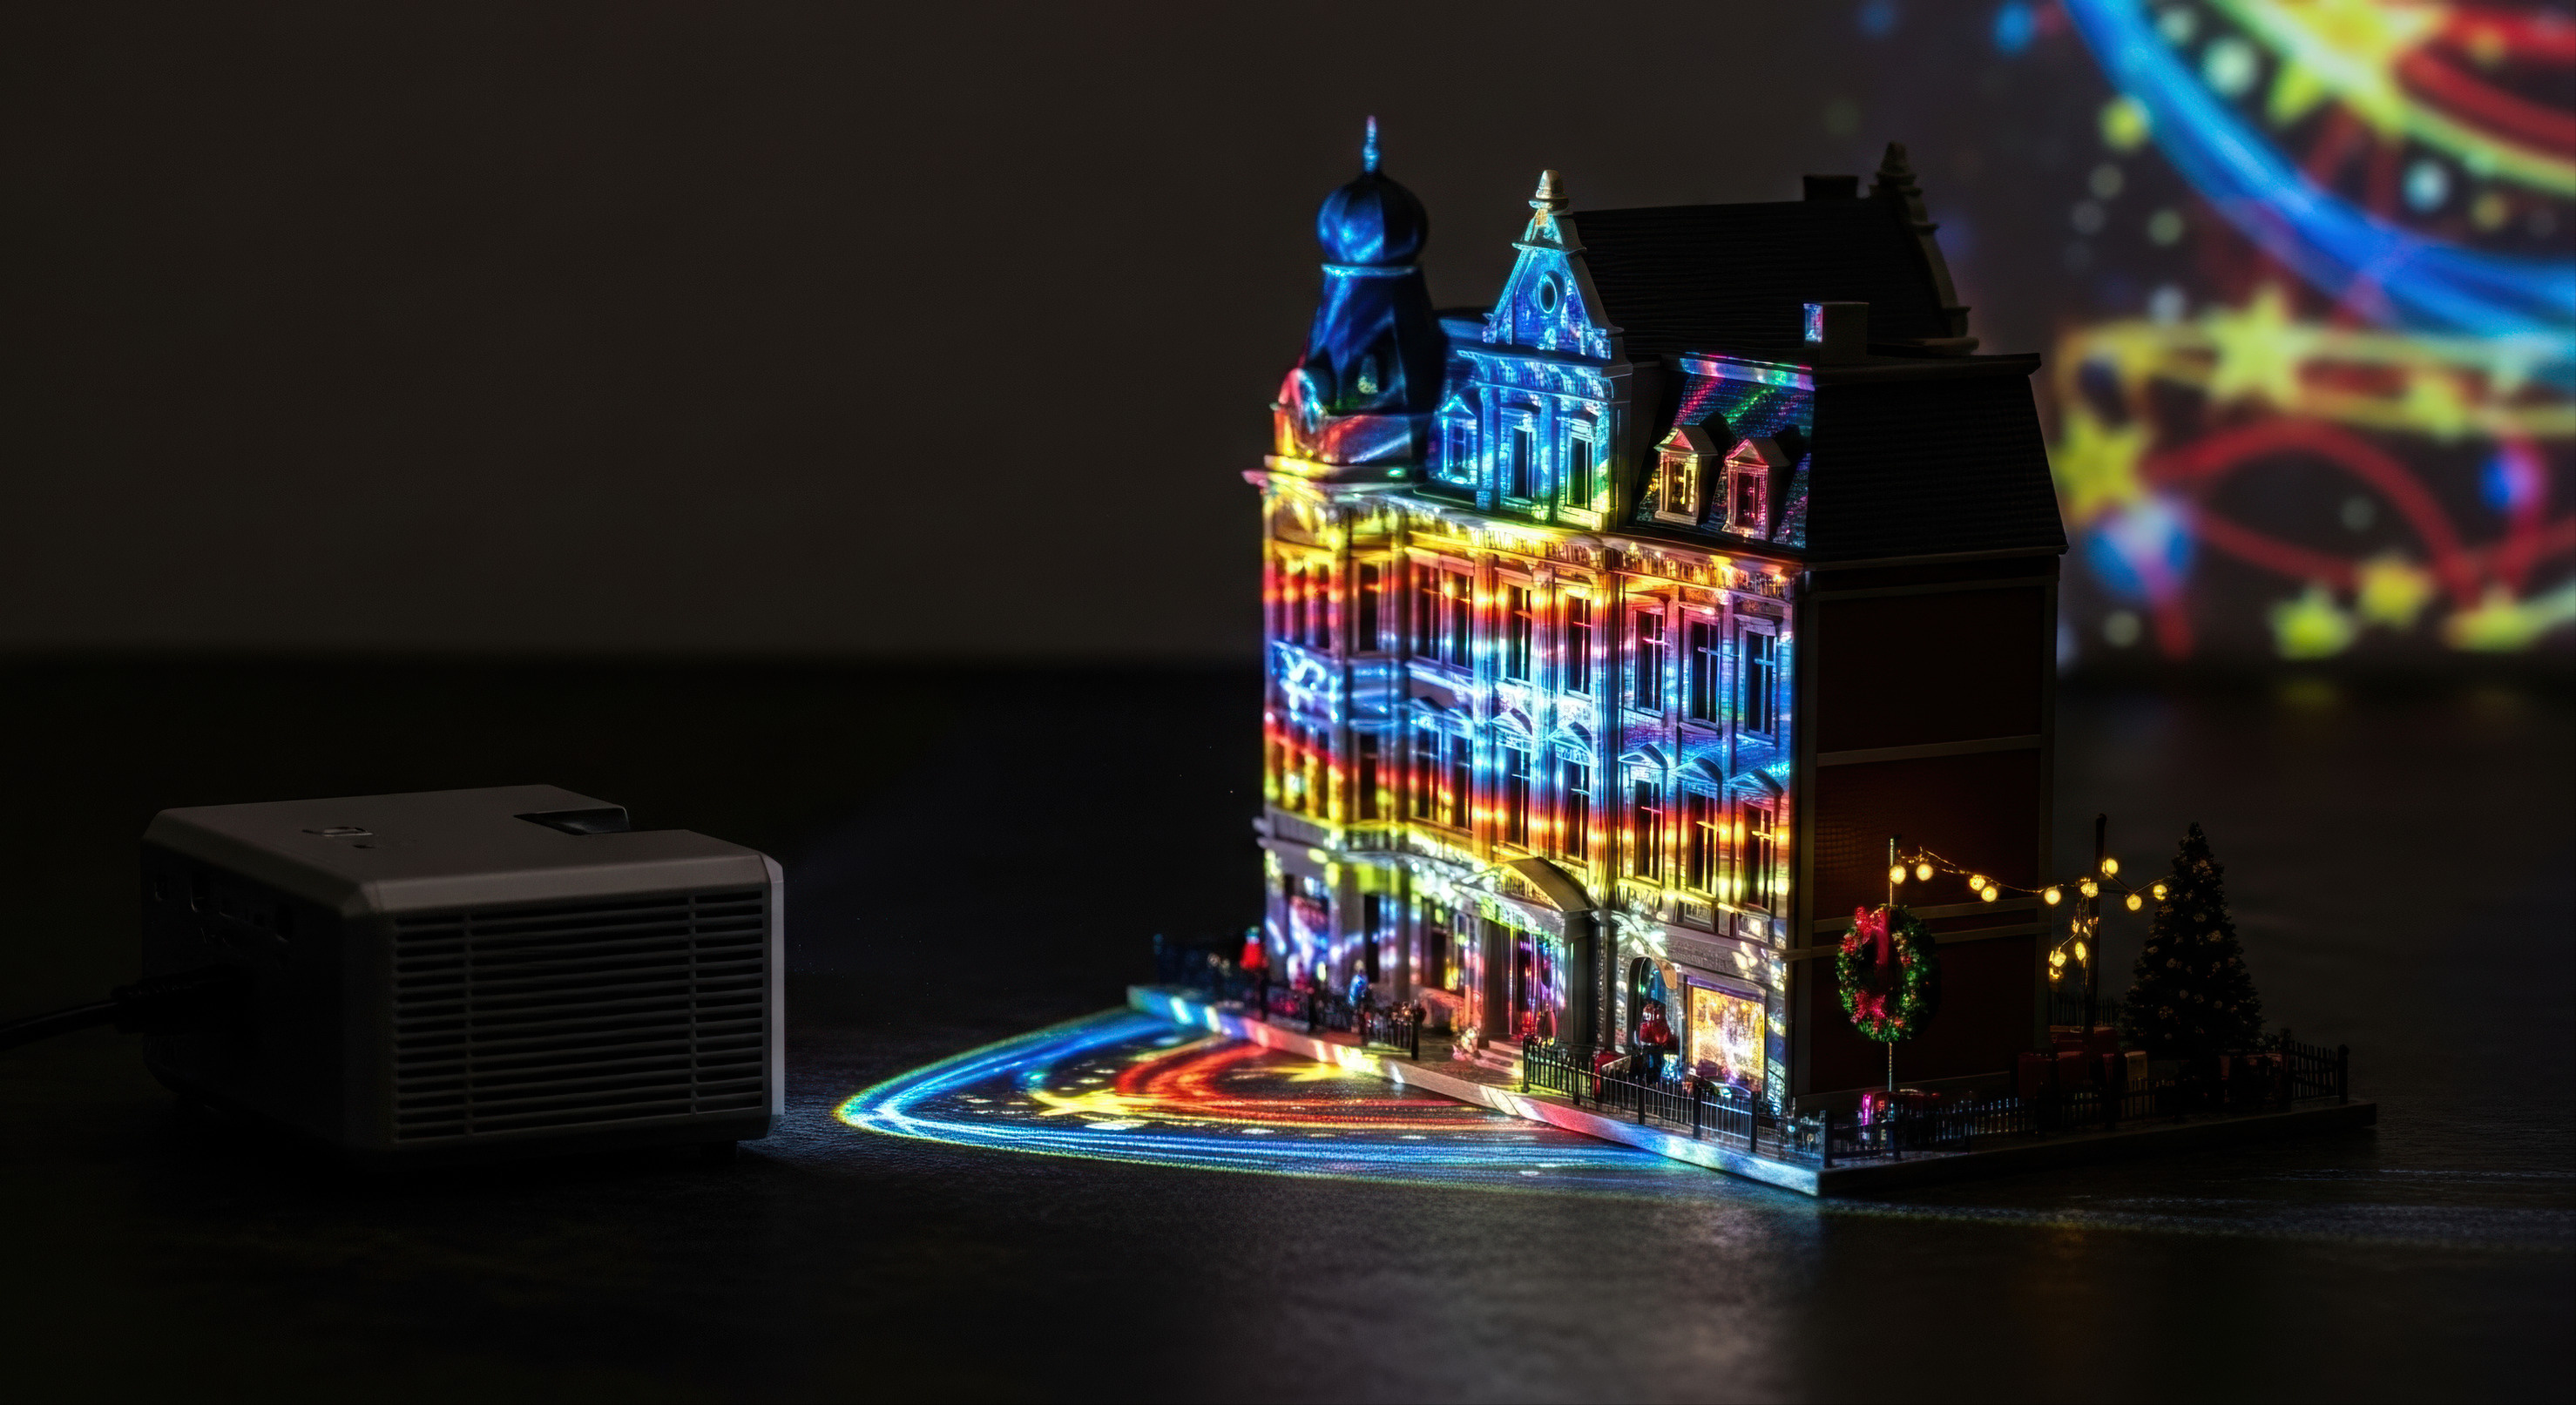
\includegraphics[width=0.5\linewidth]{thesis/figures/sample.jpeg}
    \caption{図の基本的な載せ方}
    \label{fig:basic}
\end{figure}

\verb|figure|環境の配置オプションは，希望する位置を\LaTeX に伝えるものである（表\ref{tab:floatpos}）．
複数指定すると上から順に試される．基本は\verb|[htbp]|か\verb|[tb]|でよい．

\begin{table}[htbp]
    \centering
    \caption{フロートの配置オプション}
    \label{tab:floatpos}
    \begin{tabular}{cl}\toprule
        記号 & 意味 \\ \midrule
        \texttt{h} & その場（here）に置く \\
        \texttt{t} & ページ上部（top） \\
        \texttt{b} & ページ下部（bottom） \\
        \texttt{p} & 図表専用ページ（page） \\
        \texttt{H} & 強制的にその場（\texttt{here}パッケージ） \\ \bottomrule
    \end{tabular}
\end{table}

%% ===========================================================
\section{画像サイズの指定}
\label{sec:imgsize}
\verb|\includegraphics|のオプションで，画像の大きさを複数の方法で指定できる．

\begin{description}[leftmargin=*, style=nextline]
    \item[幅で指定] \verb|[width=0.8\linewidth]|：本文幅の80\%にする（最もよく使う）．
    \item[高さで指定] \verb|[height=4cm]|：高さを4cmにする．
    \item[倍率で指定] \verb|[scale=0.5]|：元の大きさの0.5倍にする．
    \item[縦横比を保つ] \verb|[width=5cm,height=3cm,keepaspectratio]|：指定範囲に収め，比率は保つ．
\end{description}

幅の基準には，本文幅を表す\verb|\linewidth|（\verb|\textwidth|）のほか，
段組み時の段幅\verb|\columnwidth|が使える．比率で指定しておくと，
レイアウトが変わっても自動で追従するため便利である．

%% ===========================================================
\section{画像の回転とトリミング}
\label{sec:imgtrim}
\verb|angle|で画像を回転でき，\verb|trim|と\verb|clip|で周囲を切り取れる（図\ref{fig:rotate}，\ref{fig:trim}）．

\begin{figure}[htbp]
    \centering
    \begin{minipage}[b]{0.45\linewidth}
        \centering
        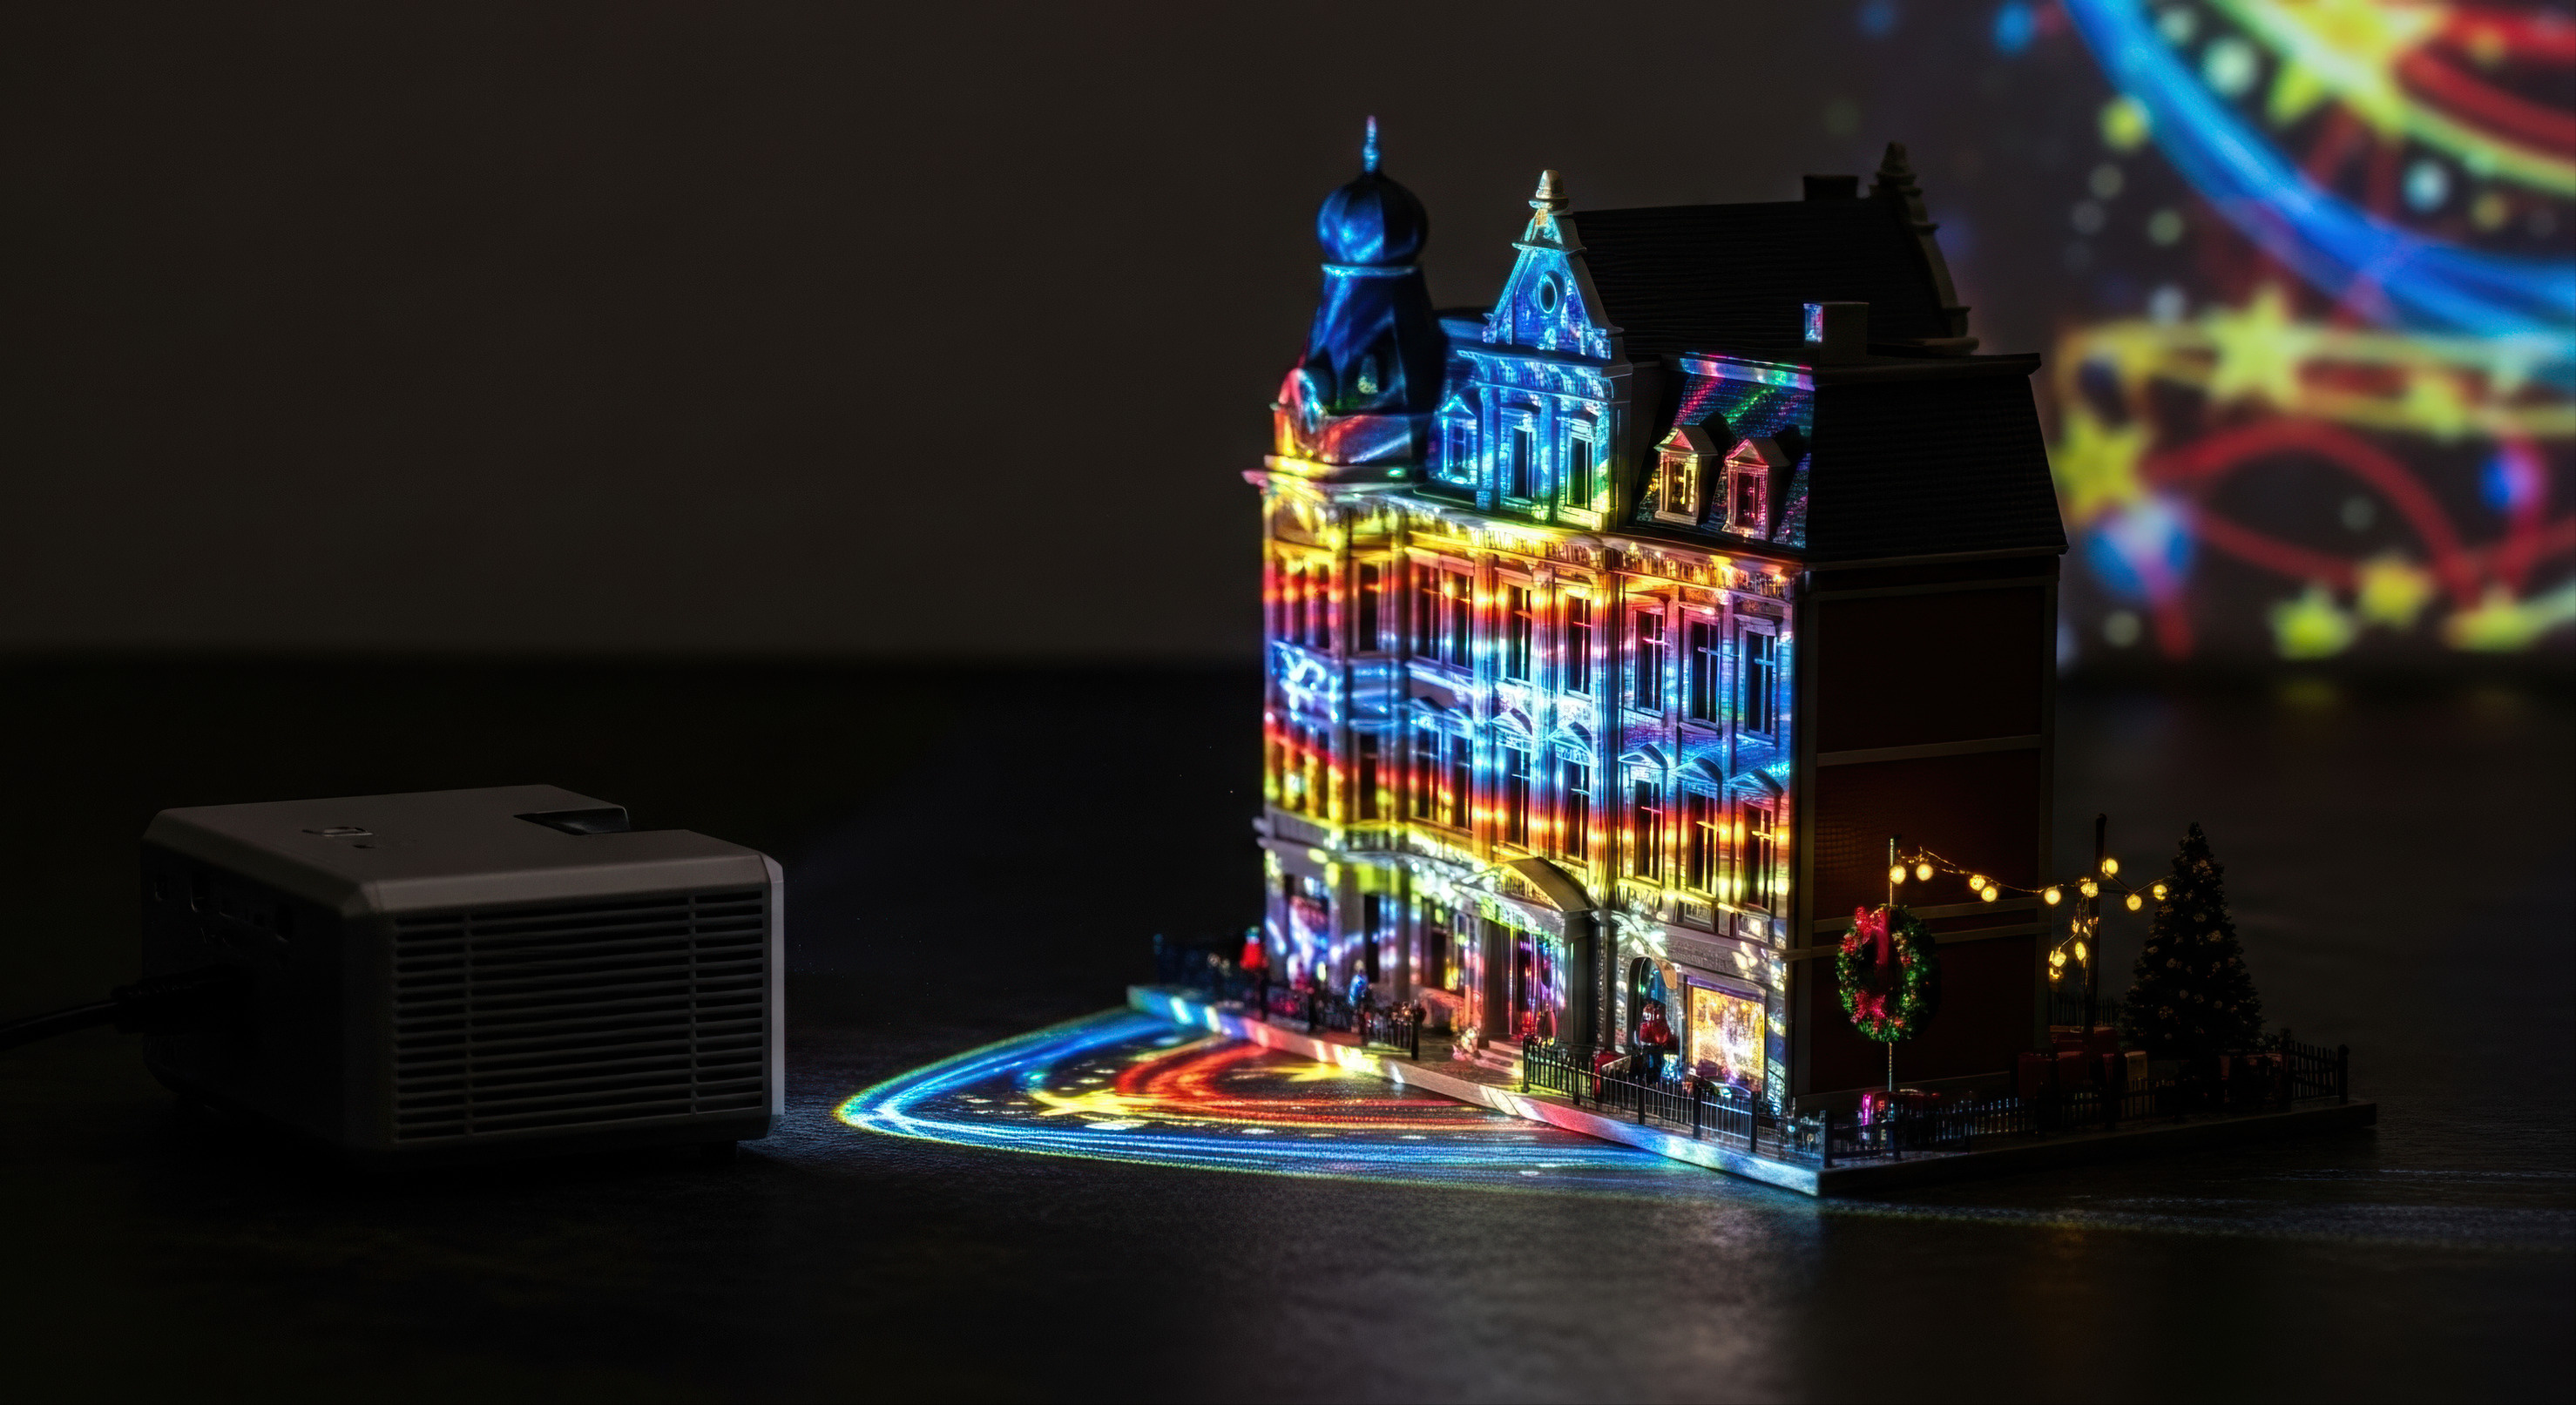
\includegraphics[width=0.5\linewidth, angle=90]{thesis/figures/sample.jpeg}
        \caption{\texttt{angle=90}で90度回転}
        \label{fig:rotate}
    \end{minipage}\hfill
    \begin{minipage}[b]{0.45\linewidth}
        \centering
        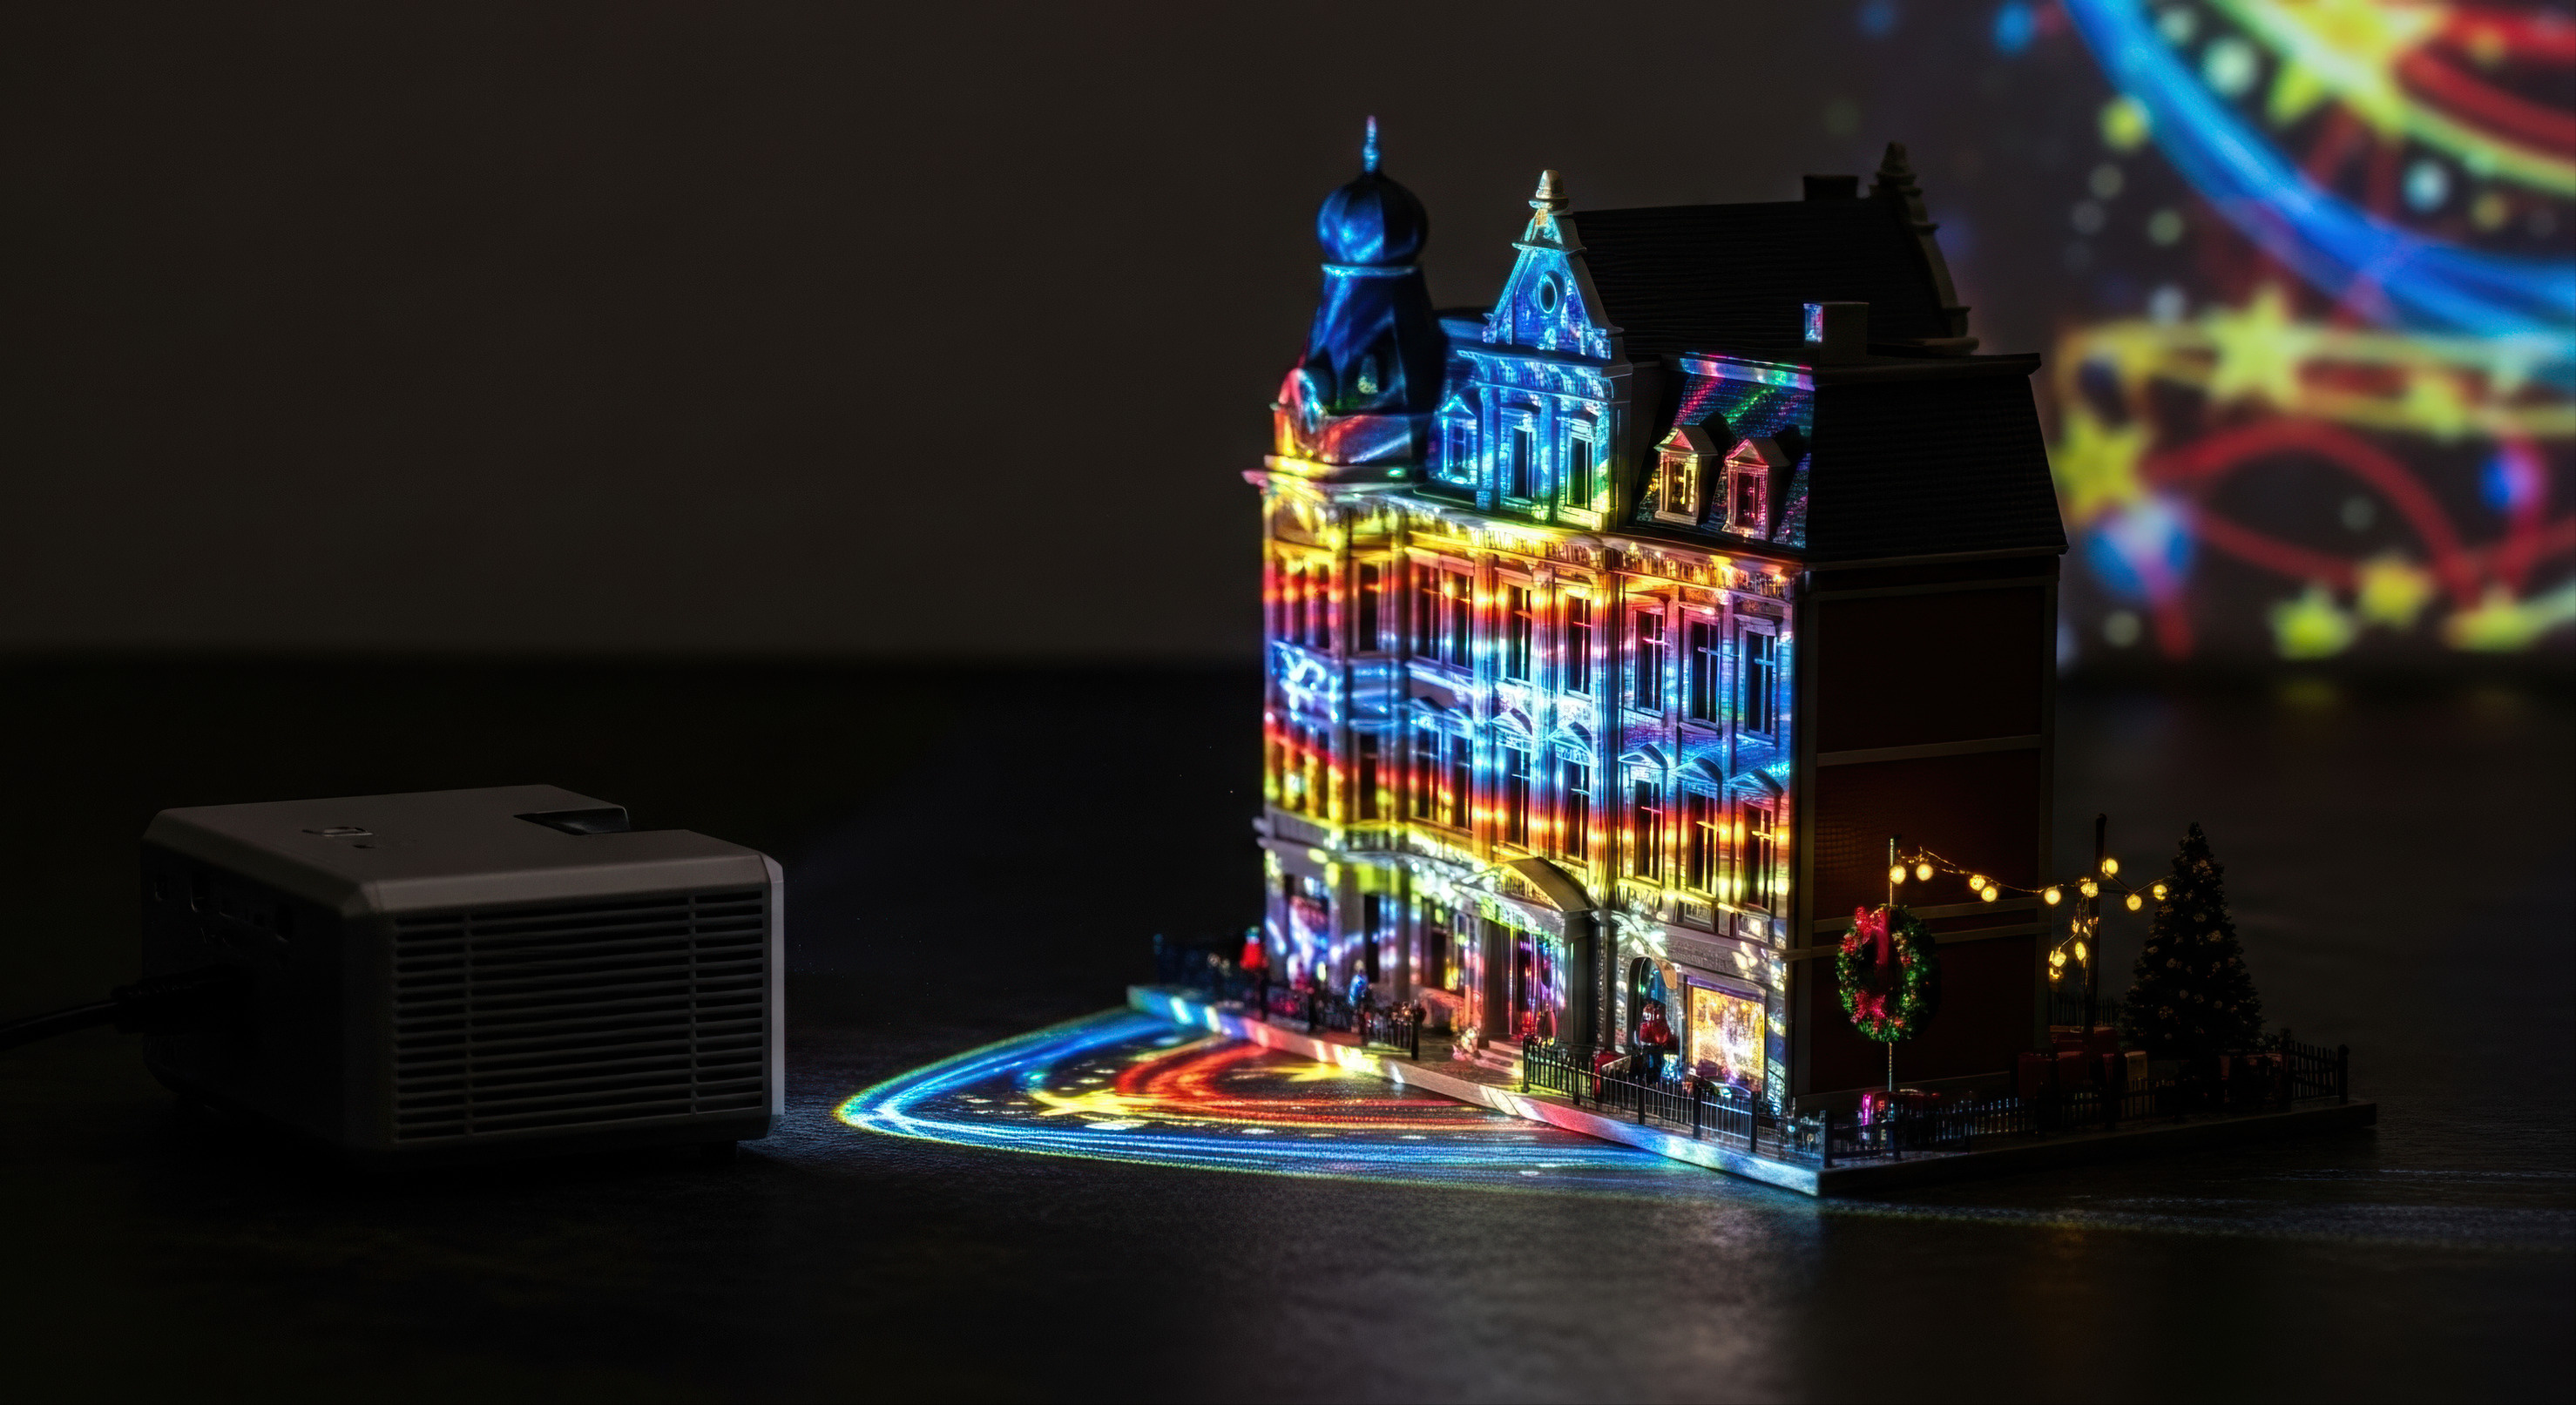
\includegraphics[width=0.6\linewidth, trim=200 200 200 200, clip]{thesis/figures/sample.jpeg}
        \caption{\texttt{trim+clip}で周囲を切り取り}
        \label{fig:trim}
    \end{minipage}
\end{figure}

\verb|trim=左 下 右 上|の順に切り取る量を指定し，\verb|clip|を付けると指定範囲外が表示されなくなる．

%% ===========================================================
\section{図を横に並べる}
\label{sec:sidebyside}
図を横に並べる方法は2通りある．キャプションを1つにまとめるか，個別に付けるかで使い分ける．

1つ目は\texttt{minipage}で並べる方法で，図\ref{fig:rotate}と図\ref{fig:trim}がその例である（個別キャプション）．
2つ目は\texttt{subcaption}で，1つの図番号の下に (a)(b)(c) と枝番号を付ける方法である（図\ref{fig:subs}）．

\begin{figure}[htbp]
    \centering
    \begin{subfigure}[b]{0.3\linewidth}
        \centering
        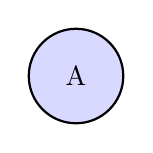
\begin{tikzpicture}\draw[thick,fill=blue!15](0,0)circle(0.6);\node at(0,0){A};\end{tikzpicture}
        \subcaption{円}\label{fig:sub-a}
    \end{subfigure}\hfill
    \begin{subfigure}[b]{0.3\linewidth}
        \centering
        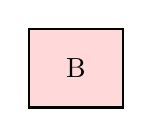
\begin{tikzpicture}\draw[thick,fill=red!15](0,0)rectangle(1.2,1.0);\node at(0.6,0.5){B};\end{tikzpicture}
        \subcaption{四角形}\label{fig:sub-b}
    \end{subfigure}\hfill
    \begin{subfigure}[b]{0.3\linewidth}
        \centering
        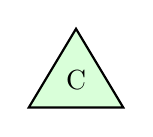
\begin{tikzpicture}\draw[thick,fill=green!15](0,0)--(1.2,0)--(0.6,1.0)--cycle;\node at(0.6,0.35){C};\end{tikzpicture}
        \subcaption{三角形}\label{fig:sub-c}
    \end{subfigure}
    \caption{subcaptionで枝番号を付けた例（図\subref{fig:sub-a}〜\subref{fig:sub-c}）}
    \label{fig:subs}
\end{figure}

%% ===========================================================
\section{本文を図に回り込ませる}
\label{sec:wrap}
\texttt{wrapfig}の\texttt{wrapfigure}環境を使うと，図の横に本文を回り込ませられる．
小さな図でページを節約したいときに有効である．

\begin{wrapfigure}{r}{0.32\linewidth}
    \centering
    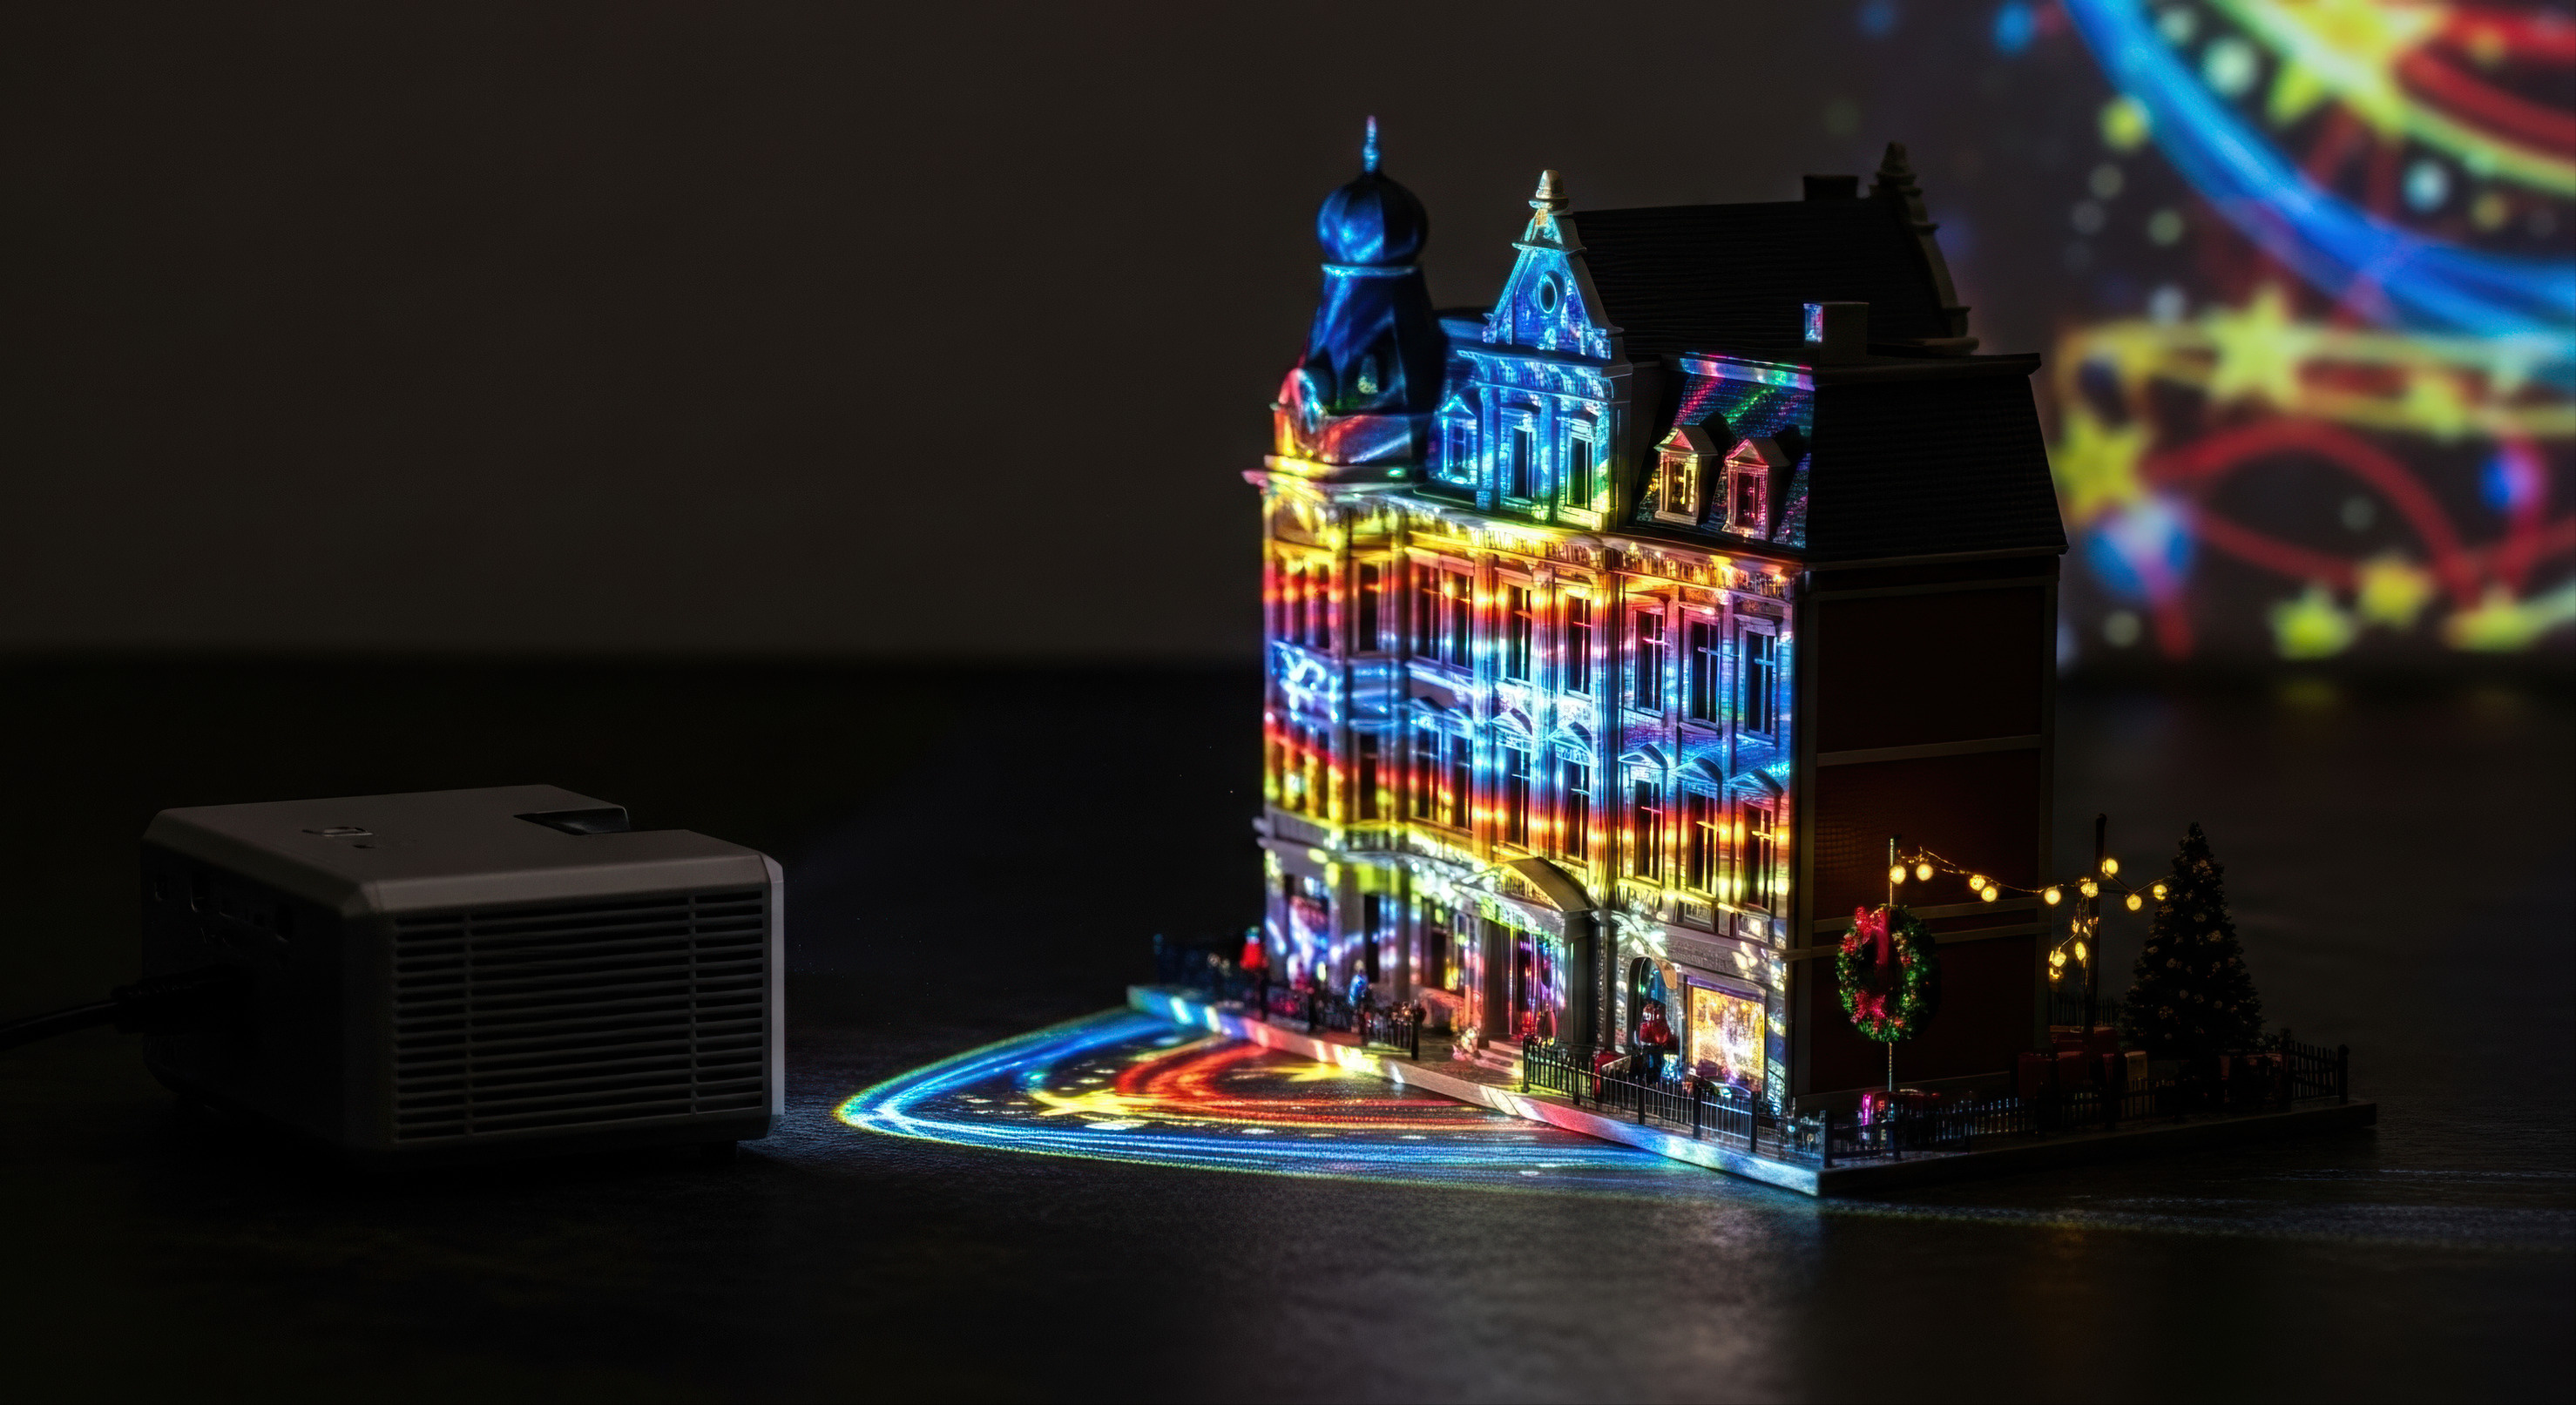
\includegraphics[width=0.9\linewidth]{thesis/figures/sample.jpeg}
    \caption{回り込みの例}
    \label{fig:wrap}
\end{wrapfigure}
\verb|\begin{wrapfigure}{r}{0.32\linewidth}|のように，第1引数で図を置く側（\texttt{r}：右，\texttt{l}：左），
第2引数で図の幅を指定する．図\ref{fig:wrap}のように，本文が図の脇に回り込んで配置される．
ただし回り込みは前後のレイアウトが乱れやすいため，使いどころには注意し，
段落の先頭付近に置くと安定しやすい．本文が十分にあると，このように自然に回り込む．
回り込ませる図はあまり大きくしすぎないことが，きれいに仕上げるこつである．

%% ===========================================================
\section{TikZ で図を描く}
\label{sec:tikz}
\texttt{TikZ}を使うと，\LaTeX 内でベクター形式の図を直接描ける．
拡大しても劣化せず，フォントも本文と統一できる（図\ref{fig:tikz}）．

\begin{figure}[htbp]
    \centering
    \begin{tikzpicture}[
        node distance=2cm,
        block/.style={draw, rounded corners, minimum width=1.8cm, minimum height=0.9cm},
        every edge/.style={draw, -{Stealth}, thick}]
        \node[block, fill=blue!10]  (in)   {入力};
        \node[block, fill=orange!15, right=of in]   (proc) {処理};
        \node[block, fill=green!10,  right=of proc] (out)  {出力};
        \draw (in) edge (proc) (proc) edge (out);
    \end{tikzpicture}
    \caption{TikZによるフロー図}
    \label{fig:tikz}
\end{figure}

%% ===========================================================
\section{pgfplots でグラフを描く}
\label{sec:pgfplots}
\texttt{pgfplots}を使うと，数値データから直接グラフを描ける（図\ref{fig:plot}）．
外部の画像を貼るより，体裁を本文と統一できる利点がある．

\begin{figure}[htbp]
    \centering
    \begin{tikzpicture}
        \begin{axis}[
            width=0.7\linewidth, height=5cm,
            xlabel={エポック}, ylabel={精度},
            legend pos=south east, grid=major]
            \addplot coordinates {(1,0.62)(2,0.74)(3,0.81)(4,0.86)(5,0.90)};
            \addlegendentry{提案手法}
            \addplot coordinates {(1,0.58)(2,0.66)(3,0.71)(4,0.75)(5,0.78)};
            \addlegendentry{従来手法}
        \end{axis}
    \end{tikzpicture}
    \caption{pgfplotsによる折れ線グラフ}
    \label{fig:plot}
\end{figure}

%% ===========================================================
\section{横向きページの大きな図表}
\label{sec:landscape}
縦幅に収まらない大きな図表は，\texttt{lscape}の\texttt{landscape}環境で
ページを横向きにすると収まりやすい（表\ref{tab:landscape}）．

\begin{landscape}
    \begin{table}[htbp]
        \centering
        \caption{横向きページに配置した表の例}
        \label{tab:landscape}
        \begin{tabular}{lcccccc}\toprule
            条件 & 指標1 & 指標2 & 指標3 & 指標4 & 指標5 & 指標6 \\ \midrule
            設定A & 0.81 & 0.79 & 0.85 & 0.88 & 0.90 & 0.77 \\
            設定B & 0.83 & 0.82 & 0.86 & 0.84 & 0.91 & 0.80 \\ \bottomrule
        \end{tabular}
    \end{table}
\end{landscape}

%% ===========================================================
\section{表の基本}
\label{sec:table}
表は\texttt{table}環境に入れ，キャプションは表の上に付ける（表\ref{tab:basic}）．
中身は\texttt{tabular}環境で組み，列指定で各列の揃え方を決める
（\texttt{l}：左揃え，\texttt{c}：中央，\texttt{r}：右揃え）．
\texttt{booktabs}の\verb|\toprule|・\verb|\midrule|・\verb|\bottomrule|で罫線を引く．
一般的な表では縦罫線を使わない方が読みやすい．

\begin{table}[htbp]
    \centering
    \caption{基本的な表}
    \label{tab:basic}
    \begin{tabular}{lcr}\toprule
        項目（左） & 区分（中央） & 値（右） \\ \midrule
        りんご & A & 120 \\
        みかん & B & 80 \\ \bottomrule
    \end{tabular}
\end{table}

%% ===========================================================
\section{セルの結合と部分罫線}
\label{sec:cellmerge}
\verb|\multicolumn|で列方向，\verb|\multirow|で行方向にセルを結合できる．
\verb|\cmidrule|を使うと，一部の列にだけ罫線を引ける（表\ref{tab:merge}）．

\begin{table}[htbp]
    \centering
    \caption{セル結合と部分罫線の例}
    \label{tab:merge}
    \begin{tabular}{lccc}\toprule
        \multirow{2}{*}{手法} & \multicolumn{2}{c}{評価指標} & \multirow{2}{*}{時間 [ms]} \\
        \cmidrule(lr){2-3}
                & 精度 [\%] & F1値 & \\ \midrule
        手法A    & 85.2 & 0.83 & 120 \\
        手法B    & 91.7 & 0.90 & 340 \\
        提案手法  & \textbf{93.4} & \textbf{0.92} & 150 \\ \bottomrule
    \end{tabular}
\end{table}

%% ===========================================================
\section{幅の制御・数値揃え・色付き表}
\label{sec:tablewidth}
\texttt{tabularx}を使うと，表全体の幅を指定し，\texttt{X}列に残り幅を自動配分できる．
長い文を含むセルは自動で折り返される（表\ref{tab:tabularx}）．

\begin{table}[htbp]
    \centering
    \caption{tabularxで幅を指定した表}
    \label{tab:tabularx}
    \begin{tabularx}{\linewidth}{lX}\toprule
        項目 & 説明 \\ \midrule
        概要 & \texttt{X}列は残りの幅を自動的に占め，長い文章でも指定幅で折り返される． \\
        補足 & 列指定の\texttt{p\{3cm\}}でも，幅を固定して折り返せる． \\ \bottomrule
    \end{tabularx}
\end{table}

数値を小数点で揃えたい場合は\texttt{siunitx}の\texttt{S}列が便利である．
また\texttt{colortbl}の\verb|\rowcolor|で行に色を付けられる（表\ref{tab:num}）．

\begin{table}[htbp]
    \centering
    \caption{数値揃え（S列）と行の色付け}
    \label{tab:num}
    \begin{tabular}{l S[table-format=3.2]}\toprule
        項目 & {測定値} \\ \midrule
        \rowcolor{blue!8}
        測定1 & 12.30 \\
        測定2 & 105.07 \\
        測定3 & 7.50 \\ \bottomrule
    \end{tabular}
\end{table}

%% ===========================================================
\section{ページをまたぐ表}
\label{sec:longtable}
行数が多くページをまたぐ表には\texttt{longtable}を用いる．
\verb|\endhead|で各ページに繰り返す見出し行を指定できる．

\begin{longtable}{cl}
    \caption{longtableによる長い表}\label{tab:long}\\
    \toprule 番号 & 内容 \\ \midrule
    \endfirsthead
    \toprule 番号 & 内容（続き） \\ \midrule
    \endhead
    \bottomrule
    \endfoot
    1 & 1行目 \\
    2 & 2行目 \\
    3 & 3行目 \\
\end{longtable}

%% ===========================================================
\section{数式}
\label{sec:math}
文中の数式は\verb|$...$|で囲む（例：$y = ax + b$）．
独立した別行立ての数式は，番号が不要なら\verb|\[ ... \]|，
番号を付けて参照するなら\texttt{equation}環境を用いる（式(\ref{eq:softmax})）．

\begin{equation}
    \label{eq:softmax}
    \mathrm{softmax}(z_i) = \frac{e^{z_i}}{\sum_{j=1}^{K} e^{z_j}}
\end{equation}

複数行で等号位置を揃えるには\texttt{align}を，番号を付けず並べるだけなら\texttt{gather}を用いる．

\begin{align}
    f(x) &= (x+1)^2 \notag \\
         &= x^2 + 2x + 1
\end{align}

場合分けには\texttt{cases}，行列には\texttt{pmatrix}（丸括弧）や\texttt{bmatrix}（角括弧）を使う．
括弧の大きさは\verb|\left|・\verb|\right|で中身に自動で合わせられる．

\begin{equation}
    \mathrm{sgn}(x) =
    \begin{cases}
        \ 1  & (x > 0) \\
        \ 0  & (x = 0) \\
        -1   & (x < 0)
    \end{cases}
    \qquad
    A = \left( \begin{matrix} a & b \\ c & d \end{matrix} \right)
\end{equation}

総和$\sum_{i=1}^{n}$，積分$\int_a^b f(x)\,dx$，極限$\lim_{n\to\infty}$，
分数$\frac{1}{2}$，平方根$\sqrt{x}$，ギリシャ文字（$\alpha, \beta, \gamma, \pi$），
上付き$x^2$・下付き$x_i$など，多くの記号が\texttt{amsmath}・\texttt{amssymb}で利用できる．
数式中で日本語や立体の語を書くには\verb|\text{...}|や\verb|\mathrm{...}|を用いる．
数式中の変数や記号は，本文中で必ずその意味を説明すること．

%% ===========================================================
\section{定義・定理環境}
\label{sec:theorem}
定義や定理は専用の環境で記述でき，章ごとに自動で採番される．

\begin{definition}[エントロピー]
    確率分布 $p = (p_1, \dots, p_n)$ のエントロピー $H(p)$ を次式で定義する．
    \begin{equation}
        H(p) = -\sum_{i=1}^{n} p_i \log p_i
    \end{equation}
\end{definition}

\begin{theorem}
    台が有限な確率分布の中で，一様分布はエントロピーを最大にする．
\end{theorem}
\begin{proof}
    Lagrangeの未定乗数法により示せる（詳細は省略する）．
\end{proof}

%% ===========================================================
\section{ソースコード}
\label{sec:code}
ソースコードは\texttt{listings}の\texttt{lstlisting}環境で掲載する（ソースコード\ref{lst:fib}）．
\verb|caption|・\verb|label|でキャプションと参照を，\verb|language|で言語を指定すると，
キーワードや文字列に自動で色が付く．論文の主張に関係する部分のみを抜粋すること．

\begin{lstlisting}[caption={Pythonによる例}, label={lst:fib}, language=Python, float=tb]
# フィボナッチ数列の第 n 項を返す関数
def fib(n):
    a, b = 0, 1
    for _ in range(n):
        a, b = b, a + b
    return a
\end{lstlisting}

文中に短いコードを埋め込むには\verb|\verb|や\verb|\texttt{}|を用いる（例：\verb|print(x)|）．
外部ファイルをそのまま読み込んで掲載するには\verb|\lstinputlisting|を用いる．

\begin{lstlisting}[language={[LaTeX]TeX}, numbers=none, frame=single]
\lstinputlisting[language=Python]{src/main.py}
\end{lstlisting}

%% ===========================================================
\section{アルゴリズム}
\label{sec:algorithm}
擬似コードは\texttt{algorithm}（フロート）と\texttt{algpseudocode}（擬似コード本体）で記述する（アルゴリズム\ref{alg:bsearch}）．

\begin{algorithm}[htbp]
    \caption{二分探索}
    \label{alg:bsearch}
    \begin{algorithmic}[1]
        \Require ソート済み配列 $A[1..n]$，探索値 $x$
        \Ensure $x$ の添字（存在しなければ $-1$）
        \State $lo \gets 1,\quad hi \gets n$
        \While{$lo \le hi$}
            \State $mid \gets \lfloor (lo + hi) / 2 \rfloor$
            \If{$A[mid] = x$}
                \State \Return $mid$
            \ElsIf{$A[mid] < x$}
                \State $lo \gets mid + 1$
            \Else
                \State $hi \gets mid - 1$
            \EndIf
        \EndWhile
        \State \Return $-1$
    \end{algorithmic}
\end{algorithm}

%% ===========================================================
\section{枠囲みと外部PDFの挿入}
\label{sec:box}
注意点やまとめは枠で囲むと目立つ．\texttt{ascmac}の\texttt{itembox}を用いた例を示す．

\begin{itembox}[l]{提出前チェックリスト}
    \begin{itemize}
        \item \verb|\ThisIsDraft|を削除したか
        \item 図表・参考文献に未参照・未定義がないか
        \item overfull が発生していないか（第\ref{sec:overfull}節参照）
    \end{itemize}
\end{itembox}

既存のPDF（アンケート用紙やデータシートなど）を付録として丸ごと挿入するには，
\texttt{pdfpages}の\verb|\includepdf|を用いる．

\begin{lstlisting}[language={[LaTeX]TeX}, numbers=none, frame=single]
\includepdf[pages=-]{appendix/questionnaire.pdf} % 全ページ挿入
\end{lstlisting}

%% ===========================================================
\section{Overfullへの対処}
\label{sec:overfull}
組版時に行が右側にはみ出す現象を overfull という．原則として overfull を起こさないよう工夫する．
発生しやすい例として，長い英単語・URL・数式・\verb|\verb|コマンドがある．
URLは\verb|\url{}|で囲む，長い英単語は適切な位置で改行を許可するなどの対処を行う．
\verb|\\|や\verb|\linebreak|による強制改行での回避はできるだけ避ける．

    \chapter{結論}
\label{chap:conclusion}

%% ===========================================================
\section{本研究のまとめ}
\label{sec:summary}
本論文では，\upLaTeX による卒業論文・修士論文の執筆を支援するテンプレートについて述べた．
第\ref{chap:writing}章では論文執筆の作法を，第\ref{chap:latex}章および第\ref{chap:float}章では
論文の執筆に必要な\LaTeX の記法を，さまざまなパターンとともに網羅的に示した．
これにより，執筆者は体裁を整える手間を抑え，内容の検討に集中できる．

結論では，このように序論（第\ref{chap:intro}章）で述べた目的に対して，
本研究で何を行い，どの程度達成できたかを簡潔に振り返る．

%% ===========================================================
\section{今後の課題}
\label{sec:future}
研究の限界や今後の課題・展望を述べることで，研究の発展性を示す．
結論が明確でない，あるいは目的の内容と結論が乖離しているものは再考を要する\cite{ipsj-sample}．
本テンプレートについては，研究分野ごとのスタイル整備や，BibTeXによる文献管理の
解説の拡充などが今後の課題として挙げられる．

    % \chapter{序論}
\label{chap:intro}

本章は，卒業論文・修士論文における「序論（はじめに）」の書き方を実例として示すものである．
序論は読者が最初に目にする章であり，論文全体の印象を大きく左右する．
一般に，\textbf{研究背景}・\textbf{問題提起}・\textbf{研究目的}・\textbf{論文の構成}の順に記述するとよい\cite{kisaragi}．
本章自体がその構成例になっている．

%% ===========================================================
\section{研究の背景}
\label{sec:background}
まず，研究対象とする分野の現状や社会的な背景を述べ，読者を研究テーマへ導く．
本テンプレートは，\upLaTeX\footnote{\LaTeX を日本語（特に縦書きや多書体）に対応させた処理系である．}
を用いて論文を執筆するための環境を提供する．
組版システムとしての\TeX は文献\cite{lamport}や文献\cite{tex}をはじめ多くの文献で解説されており，
学術論文の作成において広く利用されている．

背景の記述では，専門外の読者にも伝わるように，一般的な事柄から具体的な対象へと
順に話を進めることが望ましい．略語を用いる場合は初出時に正式名称を併記する
（例：自然言語処理 (Natural Language Processing; NLP)）．

%% ===========================================================
\section{既存研究の課題}
\label{sec:problem}
次に，既存の手法や状況にどのような課題があるのかを示す．
ここでの問題提起が，後の研究目的と対応している必要がある．
課題を述べる際は，単なる感想ではなく，先行研究の引用\cite{tex,kisaragi}に基づいて
客観的に論じることが重要である．

%% ===========================================================
\section{本研究の目的}
\label{sec:purpose}
問題提起を受けて，本研究が何を目指すのかを明確に述べる．
目的が曖昧であったり，問題提起と対応していなかったりする論文は再考を要する．
本テンプレートの目的は，論文の体裁を整える手間を最小化し，
執筆者が内容の検討に集中できる環境を提供することである．

%% ===========================================================
\section{本論文の構成}
\label{sec:structure}
最後に，以降の章で何を述べるのかを示す．
読者はこの記述を地図として論文を読み進める．

\begin{description}
    \item[第\ref{chap:intro}章\ 序論] 研究の背景・課題・目的と，本論文の構成を述べる（本章）．
    \item[第\ref{chap:writing}章\ 論文執筆の作法] 論文全体の構成や，わかりやすい文章を書くための作法をまとめる．
    \item[第\ref{chap:latex}章\ 文章作成のための\LaTeX 記法] 見出し・参照・箇条書き・引用など，文章を組み立てる基本的な記法を示す．
    \item[第\ref{chap:float}章\ 図・表・数式・コードの記法] 図の載せ方や表・数式・ソースコードなど，論文で多用する記法をパターン豊富に示す．
    \item[第\ref{chap:conclusion}章\ 結論] 本論文のまとめと今後の課題を述べる．
\end{description}

\begin{itembox}[l]{序論に含めるべき要素}
    \begin{enumerate}
        \item 研究背景：分野の現状や社会的背景
        \item 問題提起：既存手法・状況の課題
        \item 研究目的：課題に対して本研究が目指すこと
        \item 論文の構成：以降の章の概要
    \end{enumerate}
\end{itembox}
 % 自分の論文はこちらに用意する

    % ===== 後付け（参考文献） =====
    \backmatter
    % BibTeXを使う場合は thebibliography の代わりに次の2行を使う
    % \bibliographystyle{junsrt}
    % \bibliography{thesis/reference}
    \begin{thebibliography}{99}
        \bibitem{lamport}
        L. Lamport, ``\LaTeX: A Document Preparation System'', Addison-Wesley, 2nd edition, 1994.

        \bibitem{tex}
        奥村晴彦, 黒木祐介, ``改訂第9版 \LaTeXe 美文書作成入門'', 技術評論社, 2023.

        \bibitem{kisaragi}
        木下是雄, ``理科系の作文技術'', 中公新書, 1981.

        \bibitem{companion}
        F. Mittelbach, U. Fischer, ``The \LaTeX\ Companion'', Addison-Wesley, 3rd edition, 2023.

        \bibitem{ipsj-sample}
        情報処理学会論文誌ジャーナル編集委員会, ``情報処理学会論文誌ジャーナル論文の準備方法'', \url{https://www.ipsj.or.jp/journal/submit/style.html}, 参照 2026-01-15.
    \end{thebibliography}

\end{document}
